\label{sec:deadlock}
Un grupo de procesos están en estado de $deadlock$ si cada uno de ellos está esperando un evento que sólo otro proceso del grupo puede causar.
Vamos a analizar el código para demostrar que está libre de deadlocks.

Antes de eso veremos cuáles son las condiciones que debe cumplir un sistema para tener la posibilidad de llegar a un estado de deadlock, llamadas
condiciones de Coffman:
\begin{itemize}
 \item Exclusión mutua: cada recurso está asignado exactamente a un proceso o está disponible.
 \item Hold-and-wait: Los procesos que tienen asignado un recurso pueden requerir otro/s recurso/s.
 \item No-preemption: Los recursos asignados a procesos no pueden ser removidos por la fuerza.
 \item Espera circular: Debe haber una lista de dos o más procesos, cada uno de ellos esperando un recurso que tiene el anterior.
\end{itemize}

En nuestra implementación no se cumple la última condición de Coffman, por ende está libre de deadlocks.
Entonces veamos por qué no hay espera circular:

Sean $A$ y $B$ dos clientes tales que el cliente $A$ desea moverse desde la posición 1 hacia la posición 2, mientras que el cliente $B$ desea hacer lo contrario. Entonces podría suceder que el cliente $A$ se ejecute primero y haga un $lock$ sobre la posición 1 y en ese instante deja de ejecutarse y pasa a ser ejecutado el cliente $B$, que tomará un $lock$ sobre la posición 2. Cuando vuelva a ejecutarse el cliente $A$, va a requerir la posición 2 pero no va a poder porque la tiene el cliente $B$. Asimismo sucede lo mismo para el cliente $B$. Es en este caso donde sucede una espera circular y tanto el cliente $A$ con el cliente $B$ no pueden avanzar[como se puede ver el la figura \ref{fig:espera_1}

\begin{figure}[H]
	\centering
	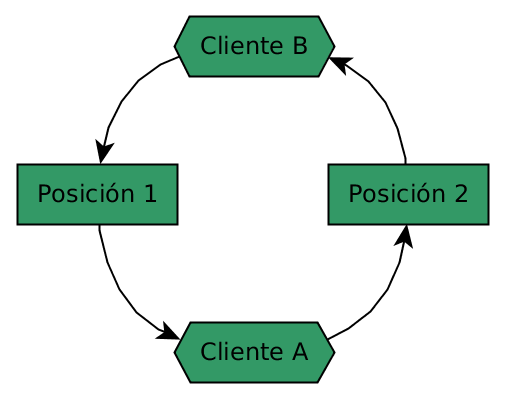
\includegraphics[scale=0.35]{imgs/espera_circular.png}
	\caption{Ejemplo de espera circular}
	\label{fig:espera_1}
\end{figure}

Para asegurarnos de que no haya espera circular en cuanto a las posiciones del aula lo que hicimos fue disponer un orden de bloqueos; esto es, tener una forma de decidir que posiciones vienen antes que otras. Dado este orden se ve que de manera que en el ejemplo de la figura \ref{fig:espera_1}, no podría suceder que el cliente $B$ tome primero el $lock$ sobre la posición 2, ya que debería tomar la menor de ambas posiciones. La relación de orden entre 2 posiciones $P_{1}$ y $P_{2}$ que nosotros definimos es la siguiente:

\begin{align*}
	P_{1} < P_{2} \iff P_{1}.fila < P_{2}.fila \lor (P_{1}.fila == P_{2}.fila \land P_{1}.columna < P_{2}.columna)
\end{align*}

También sucede en ciertos casos que un cliente puede poseer más de un recurso a la vez, esto es tierra fértil a que haya hold-and-wait, y se genere deadlock.

\begin{figure}[H]
	\centering
	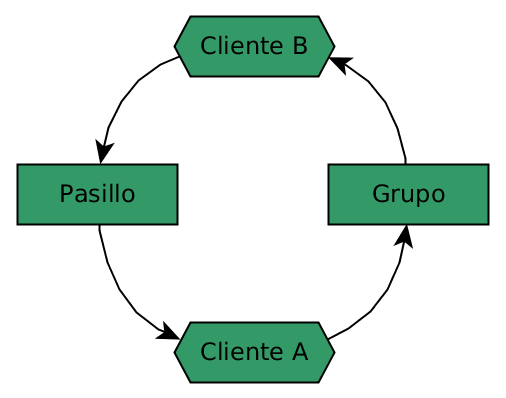
\includegraphics[scale=0.35]{imgs/deadlock_2.png}
	\caption{Ejemplo de deadlock con 2 recursos}
	\label{fig:hold_and_wait_1}
\end{figure}

En la figura~\ref{fig:hold_and_wait_1} se ve un ejemplo de deadlock con 2 recursos que puede resultar de que un cliente con un recurso quiera acceder a otro. Sin embargo, en nuestra implementación nunca sucede el caso en que un cliente pueda tener asignado el recurso del pasillo y quiera acceder al recurso del grupo. Para que esto suceda debe tener primero un lock sobre el grupo, para luego preguntar por el pasillo. Notar que hay veces que el recurso del pasillo puede estar tomado por otro cliente, pero éste eventualmente lo liberará.

Además, al momento de ingresar al grupo de evacuación, el cliente debe tomar locks en 3 recursos en simultáneo para ver si se cumplen determinadas condiciones. Sin embargo, una vez que ve si se cumplen, suelta los locks, por lo tanto, no hay deadlock.

Una variante de deadlock es el $livelock$, donde no necesariamente el sistema está en un estado del cual no puede avanzar, pero está en una serie de eventos que se repiten de manera cíclica. Esto puede afectar a nuestro sistema cuando un cliente rebelde no se acerca a la salida, y como el grupo de evacuación debe esperar a que haya 5 personas en el grupo o sean los últimos del aula entonces no pueden evacuar mientras este cliente no salga. Sin embargo, vamos a suponer que los clientes son personas lógicas y desean ser evacuados, por lo tanto eventualmente alcanzará la salida. Con esta suposición salvamos el riesgo de livelock.